\documentclass[main]{subfiles}

\begin{document}

\begin{theorem}
For every group $G$, there is a connected two dimensional CW complex $X$ with $\pi_1(X)=G$
\end{theorem}

\begin{proof}
We can always find a surjection from a free group $F$ to $G$, suppose $F$ is generated by $g_\alpha$'s, and the kernel $K$ is generated by $r_\beta$'s, i.e. $F$ has a group presentation $\langle g_\alpha|r_\beta\rangle$, then define $X$ to be $\bigvee_{\alpha}S^1_\alpha$ attached with cells $e^2_\beta$'s along each word $r_\beta$
\end{proof}

\begin{definition}
Cayley graphs, Cayley complexes
\end{definition}

\begin{definition}
A \textbf{graph}\index{Graph} $G$ is a one dimensional CW complex, a \textbf{tree}\index{Tree} $T$ is a contractible graph, $T\subseteq G$ is maximal if $T$ contains all vertices, note that in a tree there is a unique path between two vertices
\end{definition}

\begin{proposition}
Let $X$ be a connected graph, any tree in $X$ is contained in a maximal tree, in particular, $X$ has a maximal tree
\end{proposition}

\begin{proof}
Let's prove more generally any subgraph $X_0$ is the deformation retraction of subgraph $Y$ which contains all the vertices \par
Construct $X_0\subseteq X_1\subseteq X_2\subseteq\cdots$ as follows, $X_{i+1}$ is obtained by adding the closures of all the edges that connected to $X_i$, $X=\bigcup_{i}X_i$, since $X$ is path connected, let $Y_0=X_0$, and construct $Y_0\subseteq Y_1\subseteq Y_2\subseteq\cdots$ as follows, for any vertex in $X_{i+1}-X_i$, choose one edge that connects to $Y_i$, and add the closure, so we have $Y_{i+1}$ from $Y_i$, it is easy to see the $Y_{i+1}$ deformation retracts onto $Y_i$, so $Y=\bigcup_i Y_i$ deformation retracts onto $Y_0=X_0$ \par
If $X_0=T$ is a tree, so is $Y$ since $Y$ deformation retracts onto $T$ which is contractible
\end{proof}

\begin{proposition}[Free basis for connected graphs]\label{Free basis for connected graphs}
For a connected graph $X$ with maximal tree $T$, for any edge $e_\alpha\in X-T$, there is a corresponding loop $f_\alpha$ goes from $x_0$ to one endpoint of $e_\alpha$, across $e_\alpha$ to the other, and go back to $x_0$, $\pi_1(X,x_0)$ is a free group generated by $f_\alpha$
\end{proposition}

\begin{proof}
Consider $X\to X/T$ which is a homotopy equivalence
\end{proof}

\begin{theorem}
Any subgroup of a free group is also free
\end{theorem}

\begin{proof}
Let $F$ be a free group, there exists a graph $X$ such that $\pi_1(X)=F$ by just taking the wedge sum of circles at $x_0$, let $G\leq F$ be a subgroup, then there exists a covering $Y\xrightarrow{p}X$ such that $p_*(\pi_1(Y,y_0))=G$, thus $\pi_1(Y,y_0)\cong G$, and since $Y$ is a covering of $X$, $Y$ is also a graph, by Proposition \ref{Free basis for connected graphs}, $G\cong\pi_1(Y)$ is free
\end{proof}

\begin{definition}
A \textbf{complete graph}\index{Complete graph} $K_n$ consists of $n$ vertices and all possible edges
\begin{figure}[h!]
\centering
\begin{tikzpicture}
\foreach \i in {0,1,...,4}
{
\coordinate (\i) at ($cos(72*\i)*(1,0)+sin(72*\i)*(0,1)$);
\filldraw (\i) circle (0.02);
}
\foreach \i in {0,1,...,4}
{
\foreach \j in {\i,...,4}
{
\draw (\i)--(\j);
}
}
\end{tikzpicture}
\caption{$K_5$}\label{K5 complete graph}
\end{figure}
\textbf{Complete bipartite}\index{Complete bipartite} graphs are $K_{n,m}$ with $n,m$ vertices on each side and all possible edges between them
\begin{figure}[h!]
\centering
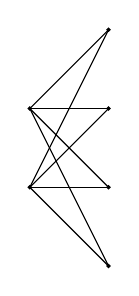
\begin{tikzpicture}
\foreach \i in {1,2}
{
\filldraw (0,\i) circle (0.02);
}
\foreach \i in {0,1,2,3}
{
\filldraw (1,\i) circle (0.02);
}
\foreach \i in {1,2}
{
\foreach \j in {0,1,2,3}
{
\draw (0,\i)--(1,\j);
}
}
\end{tikzpicture}
\caption{$K_{2,4}$}\label{K2,4 complete bipartite graph}
\end{figure}
\end{definition}

\begin{definition}
$G$ is $k$ vertex connected if $G$ has more than $k$ vertices and remain connected when removing less than $k$ vertices
\end{definition}

\begin{proposition}
Every convex polytope can be represented by a $3$ vertex connected planar graph
\end{proposition}

\begin{remark}
A graph embedded in the plane through different ways may have different dual graphs
\begin{figure}[ht!]
\centering
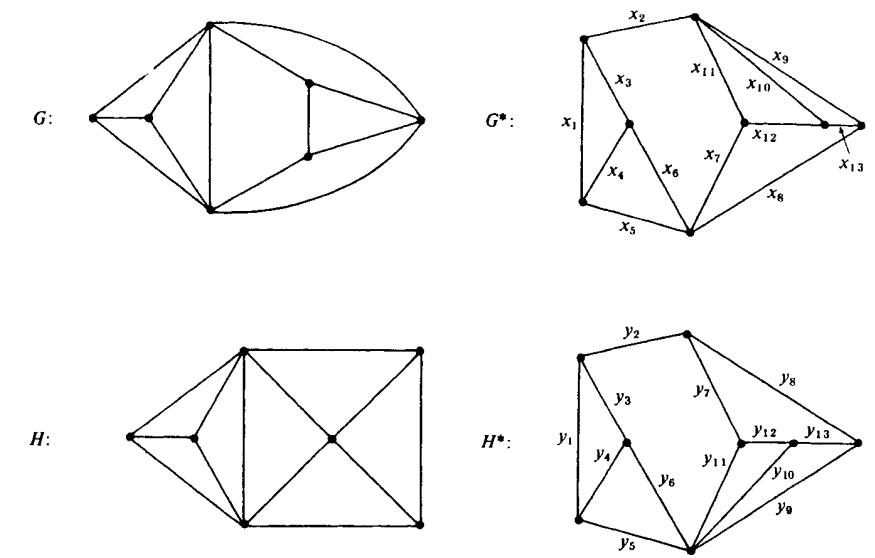
\includegraphics[scale=0.3]{Pictures/Different_dual_graphs.png}
\caption{Different dual graphs for different planar embeddings of the same graph}\label{Different dual graphs}
\end{figure}
However, if the graph is $3$ vertex connected, then the dual graph will be canonical
\end{remark}

\end{document}